\chapter{Hired Guns}

This lecture returns to the question left open by the discussion of Locke: if political authority rests on consent, what are the limits on what even a majority may rightly authorize? The movement of the hour is carefully staged. We begin with taxation and conscription, where consent seems to authorize burdens imposed by law; we then turn to military recruitment, where market exchange enters; and finally we move to reproduction and surrogacy, where the same framework of consent and exchange reaches into a more intimate domain. The lecture does not settle the issue once and for all. It sharpens it by showing that objections to markets can arise in two distinct ways: through tainted consent and through the corruption or misvaluation of the good being exchanged.

\section{From Locke to Conscription}

Sandel opens by recalling the result of the previous lecture. On Locke's view, taxation does not require the fresh consent of each individual at the moment the tax is collected. What matters is the prior act of joining political society and accepting the authority of majority rule. That starting point matters because the lecture now asks for the harder case. If prior consent can authorize taxation, can it also authorize conscription?

\begin{equation}
\text{prior consent to join political society} \Longrightarrow \text{being bound by majority rule}
\end{equation}

\begin{equation}
\text{taxation without fresh individual consent} \not\Rightarrow \text{conscription is illegitimate}
\end{equation}

The tension is immediate. If we own ourselves, and if self-possession includes authority over our own bodies and lives, then compulsory military service seems to violate precisely the right Locke is meant to protect. Sandel therefore asks what Locke would say about a government that orders citizens to fight and risk death in war.

Locke's answer, as Sandel presents it, turns on a distinction between legitimate authority and arbitrary power. The issue is not whether government may command at all; the issue is whether it rules by law or by arbitrary will.

\begin{align}
\text{legitimate authority} &\Longrightarrow \text{non-arbitrary rule of law},\\
\text{command a soldier into danger} &\text{ may be legitimate},\\
\text{take a penny arbitrarily} &\text{ is corrupt.}
\end{align}

The sergeant example makes the point vivid. A sergeant may order a soldier into a place where he is almost certain to die, and a general may punish desertion with death. But neither may take the soldier's money merely because he has power over him. The first belongs to rightful military authority; the second is arbitrary and therefore corrupt. That is the Lockean limit.

\subsection{Question \& Answer}

\paragraph{Question.} If we own ourselves, how can government ever command us to fight?

\paragraph{Answer.} Sandel's Lockean answer is that self-ownership does not cancel the force of prior consent to political society. Consent does not mean that each order must be separately approved. It means that authority can bind us so long as it operates through general law rather than arbitrary will. Conscription is therefore not ruled out simply because it reaches our lives; it is ruled out only if it takes an arbitrary form.

This answer does not resolve the deeper question. It opens it. Sandel immediately asks why consent should be such a powerful moral instrument in creating political authority and political obligation. The rest of the lecture begins to investigate that question through a concrete case.

\section{Recruitment Options and the Civil War Hybrid}

The concrete case is military recruitment during the Iraq war. Sandel asks us to consider a state that cannot meet its recruiting targets and must decide how to fill its ranks. The lecture here becomes explicitly comparative: several institutional forms are put side by side so that the moral logic of each can be tested.

\begin{figure}[h]
\centering

\includegraphics[width=0.82\textwidth]{lecture_05_figure_02.png}
\caption{Recruitment options: higher pay or a draft. The third option, outsourcing, enters in the spoken continuation rather than on the slide itself.}
\end{figure}

The slide preserves the first two options actually shown in class, and the transcript adds the third. Taken together, they give the full recruitment menu:

\begin{equation}
\text{recruitment shortfall} \Longrightarrow
\begin{cases}
\text{increase pay and benefits},\\
\text{conscription by lottery},\\
\text{outsource to mercenaries}.
\end{cases}
\end{equation}

The point of this menu is not merely to list policy alternatives. It begins to trace a path from state compulsion to market allocation. Sandel soon adds an intermediate case that is morally more revealing than any simple abstract contrast between draft and volunteer service: the Civil War system of conscription with a buyout provision.

\begin{equation}
\text{conscription}
\to
\text{Civil War buyout}
\to
\text{all-volunteer army}
\to
\text{outsourcing}
\end{equation}

This chain is not a historical law. It is a reconstruction of the lecture's logical sequence. We begin with a draft, then allow substitution for pay, then generalize the market logic into a paid army, and then ask whether the same principle would support hiring outside professionals or mercenaries. Sandel's method is to move step by step and ask whether each added layer of market freedom preserves justice or distorts it.

\begin{figure}[h]
\centering
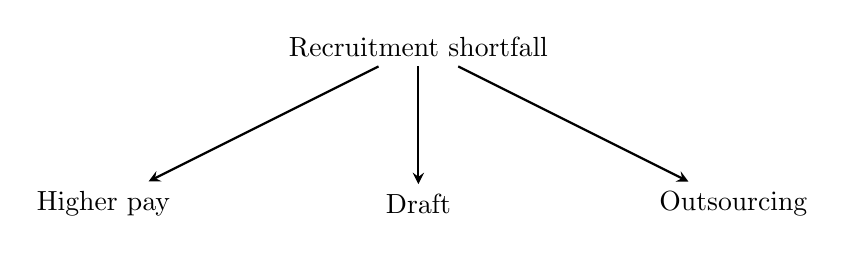
\begin{tikzpicture}[>=stealth, thick]
\node (root) at (0,0) {Recruitment shortfall};
\node (pay) at (-4,-2) {Higher pay};
\node (draft) at (0,-2) {Draft};
\node (out) at (4,-2) {Outsourcing};
\draw[->] (root) -- (pay);
\draw[->] (root) -- (draft);
\draw[->] (root) -- (out);
\end{tikzpicture}
\caption{Transcript-backed reconstruction of the recruitment decision tree.}
\end{figure}

The Civil War example sharpens the issue because it combines law and market. One is drafted, but one may hire a substitute. Sandel's students immediately see that such a system is not merely about military necessity. It is also about who bears risk, who may buy exemption, and what kind of good military service is.

\section{Coercion, Inequality, and the All-Volunteer Army}

The first criticism emerges in stages. Liz objects that paying a substitute puts a price on human life. Jason replies in libertarian fashion that there is no imposed price here: a person may decide for himself what risk is worth taking, and if he accepts the money voluntarily, the exchange seems unobjectionable.

The lecture then moves to the stronger objection made by Sam and reinforced by Raul. The problem is not simply that money enters the picture. The problem is that background inequality may make the apparently voluntary exchange not fully free at all.

\begin{equation}
\text{free consent} = \text{voluntariness} + \text{adequate information}
\end{equation}

\begin{equation}
\text{severe background inequality} \Longrightarrow
\text{apparently voluntary exchange may be partly coercive}
\end{equation}

The force of the argument lies in Sandel's example. For Carnegie, the buyout price is negligible; for a poor laborer, the same payment can be decisive. The money functions differently because the surrounding social circumstances differ.

\begin{equation}
\text{for Carnegie: } \text{\$300 or \$500 is an escape from service},\qquad
\text{for a poor laborer: the same sum is an inducement to fight}
\end{equation}

\paragraph{A worked example.} We can write the objection in the sequence Sandel elicits from the room:
\begin{enumerate}
\item The hybrid system begins with equal legal exposure to the draft.
\item It then introduces money as a way to reassign the burden.
\item Under unequal social conditions, the same payment is optional for the wealthy and urgent for the poor.
\item Therefore the resulting exchange has the form of consent without the substance of equal freedom.
\end{enumerate}

Emily then makes the decisive move of the first half of the lecture. Even if one grants the coercion objection in the Civil War case, why stop there? Does not the same objection press against the all-volunteer army, which also recruits disproportionately from those with fewer economic options? In that moment, Sandel prevents the class from treating the Civil War system as a morally isolated curiosity. The objection becomes structural.

\subsection{Question \& Answer}

\paragraph{Question.} When does a voluntary exchange stop being fully free because inequality is doing the work?

\paragraph{Answer.} The lecture's answer is not a numerical threshold. It is a structural point. Exchange ceases to be fully free when the background distribution of opportunity so constrains one side that the choice to sell labor or assume risk reflects necessity more than willing endorsement. Sandel does not yet specify exactly which inequalities count as disqualifying; instead, he identifies that question as one of the central philosophical tasks opened by the case.

At this point the lecture could have stayed within the coercion frame. Instead, it turns again.

\section{Patriotism, Civic Obligation, and Market Allocation}

Once Emily extends the coercion argument to the volunteer army, Sandel allows a different line of thought to emerge. Perhaps the deepest problem with market allocation in military service is not merely unfairness. Perhaps military service is bound up with patriotism and civic obligation, and for that reason should not be treated as just another wage relation.

Jackie argues that service motivated by patriotism is morally and practically superior to service motivated by money alone. Philip responds that mercenaries may perform just as effectively as patriotic citizens. Sandel's intervention is crucial here. He points out that the phrase ``all-volunteer army'' can obscure what is really at stake: a volunteer army, in current usage, is a paid army. Once that is seen clearly, the question becomes sharper. If patriotism ought to be primary, does that support the paid military we have, or does it point back toward conscription?

The lecture now explicitly separates two objections that had previously been intertwined in the discussion:

\begin{equation}
\text{objection}_1=\text{coercion under inequality},
\qquad
\text{objection}_2=\text{civic obligation / patriotism}
\end{equation}

The first says that background inequality can taint apparently free exchange. The second says that military service may be the wrong kind of good to allocate through market exchange in the first place. It is a question not only of fairness, but of fitting valuation.

Sandel then formulates the two questions that the whole first half of the lecture has generated:

\begin{equation}
\text{Question 1: what inequalities undermine free labor exchange?}
\end{equation}

\begin{equation}
\text{Question 2: what are the obligations of citizenship?}
\end{equation}

These questions are not answered here. Their importance lies precisely in the fact that they survive the case that produced them. The lecture's method is cumulative: discussion of one institutional choice opens a more general philosophical problem, and that problem is then carried forward into a new domain.

\section{From Military Service to Markets in Reproduction}

The bridge to the second half is abrupt in topic but continuous in logic. Sandel asks whether one should be able to bid for a baby that is up for adoption. That question sounds at first like a separate issue, but it is in fact the same issue in a new setting. We are again asking whether market exchange can rightly govern a domain whose moral meaning may exceed use, preference, and price.

He first turns to egg markets and sperm markets. Advertisements solicit highly specified egg donors and offer enormous sums for particular traits. On the sperm side, Sandel describes California Cryobank as a for-profit institution that screens heavily, markets prestige, compensates donors per specimen, and openly recruits traits the market finds attractive. The details matter because they force the question into view: if reproductive capacities can be bought and sold, what exactly is being valued, and in what mode?

The lecture does not pause long over these examples. Their main role is preparatory. They widen the field from military labor to reproductive labor and make the next case, commercial surrogacy, feel like the next natural step rather than a disconnected controversy.

\section{Surrogacy, Contract, and Tainted Consent}

The Baby M case gives the second half its structure. The Sterns, unable to have a child without medical risk, enter into a contract with Mary Beth Whitehead. She agrees to be artificially inseminated with William Stern's sperm, bear the child, and surrender the baby to the Sterns in exchange for a fee plus expenses.

\begin{equation}
\text{payment} + \text{artificial insemination} + \text{birth} \Longrightarrow \text{transfer of child to the Sterns}
\end{equation}

The first response Sandel draws from the room is straightforwardly contractual. Patrick states the principle cleanly: a deal is a deal. If competent adults knowingly and voluntarily entered the agreement, then the agreement should be enforced.

The first objection to this position does not deny the importance of consent. It qualifies it. Evan argues that the surrogate mother could not know in advance how she would feel about the child she would bear. In that respect the consent, though voluntary, was not fully informed.

\begin{equation}
\text{consent can fail through coercion}
\qquad \text{or} \qquad
\text{consent can fail through inadequate information}
\end{equation}

\begin{equation}
\text{pre-birth consent} \not\Rightarrow \text{fully informed consent}
\end{equation}

That distinction is one of the lecture's most important formal clarifications. Earlier, in the military-service discussion, consent was threatened by inequality and coercion. Here, the pressure comes from imperfect information. The two cases differ, but the structure is parallel.

Anna adds a stronger claim about natural bond and the child's right to the biological mother. Kathleen pushes back by returning to the contractual line: later emotional change does not undo a valid agreement. Andrew then introduces a different objection entirely. The problem, he says, is not merely lack of information. It is that surrogacy looks too much like baby-selling, too much like turning persons and parental claims into objects of trade.

\subsection{Question \& Answer}

\paragraph{Question.} Can a surrogacy contract be fully voluntary if the mother cannot yet know the bond she will form with the child?

\paragraph{Answer.} Sandel's answer is that voluntariness and informedness must be distinguished. A person may enter a contract without overt pressure and yet still lack the relevant knowledge needed for genuinely informed consent. In surrogacy, the court's concern is not that Whitehead was forced in the usual sense, but that she was asked to make an irrevocable choice before she could know the emotional reality of bearing and surrendering the child.

Vivian's comparison between sperm donation and surrogacy deepens the same point. On her view, the biological and temporal investment of pregnancy cannot be assimilated to sperm donation. The goods and services are morally unequal, because the bond and the labor are unequal.

\section{Commodification and the Limits of Market Reason}

The discussion then moves from classroom debate to the reasoning of the courts. Sandel notes that the lower court found the contract enforceable, while the New Jersey Supreme Court did not. The stable content of the court's reasoning, and the part Sandel preserves, is that two different arguments speak against enforcement: insufficiently informed consent and commodification.

\begin{figure}[h]
\centering

\includegraphics[width=0.82\textwidth]{lecture_05_figure_03.png}
\caption{Quote framing the commodification objection to surrogacy.}
\end{figure}

The slide fixes the tone of the second objection. Even without reproducing its full wording in the prose, we can represent its core thought as follows:

\begin{equation}
\text{profit motive predominates and governs the transaction}
\end{equation}

And we can summarize the court's two lines of objection schematically:

\begin{equation}
\text{objection}_1=\text{tainted consent},
\qquad
\text{objection}_2=\text{commodification / dehumanization}
\end{equation}

\begin{figure}[h]
\centering
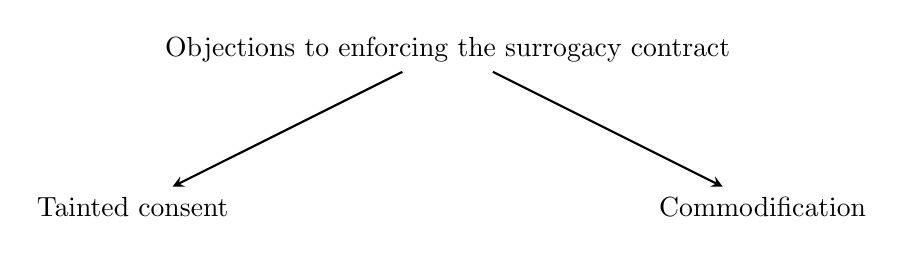
\begin{tikzpicture}[>=stealth, thick]
\node (root) at (0,0) {Objections to enforcing the surrogacy contract};
\node (consent) at (-4,-2) {Tainted consent};
\node (commod) at (4,-2) {Commodification};
\draw[->] (root) -- (consent);
\draw[->] (root) -- (commod);
\end{tikzpicture}
\caption{A note-native reconstruction of the lecture's two-part analysis.}
\end{figure}

The commodification objection is more elusive than the consent objection. Sandel says so explicitly. Its point is not simply that one party was misinformed or pressured. It is that childbearing and parental relation may be degraded when treated as items to be purchased.

To give this unease philosophical clarity, Sandel turns to Elizabeth Anderson. Her claim is that surrogacy contracts can convert women's labor into alienated labor. Pregnancy normally aims toward an emotional bond between mother and child; the contract requires that bond to be repressed or redirected.

\begin{equation}
\text{surrogacy contract} \Longrightarrow \text{alienated labor}
\end{equation}

From this point the lecture broadens. The issue is no longer only surrogacy. It is whether some goods are properly valued in ways other than use and price.

\begin{equation}
\text{some goods are not properly valued merely by use or price}
\end{equation}

Anderson's list gives Sandel a vocabulary for these non-market modes of valuation:

\begin{equation}
V_{\text{non-market}}
=
\{\text{respect},\ \text{appreciation},\ \text{love},\ \text{honor},\ \text{awe},\ \text{sanctity}\}
\end{equation}

The closing example of Cecil Jacobson reinforces the same thought from a different angle. One may criticize the case as a failure of informed consent, but Sandel also suggests a deeper unease. Ellen Goodman's line that fatherhood should be something one does, not something one donates, points toward the same question that Andrew raised and Anderson clarifies: are there goods whose meaning is damaged when they are translated into market terms?

\section{Summary}

The lecture begins with Locke and ends with a question Locke alone cannot answer. Prior consent may justify political authority, but once market exchange enters the picture we need further distinctions. In military service, Sandel extracts two objections to markets: first, inequality can corrupt apparently voluntary choice; second, military service may be connected to patriotism and civic obligation in a way that resists market valuation. In surrogacy, the same two-part structure returns in a new form: consent may be tainted by lack of information, and the good being exchanged may be degraded by being treated as a commodity.

What the lecture leaves us with is not a single doctrine but a sharpened field of inquiry. When is consent morally sufficient? When is a market exchange unfair because background conditions are unequal? And when, even absent coercion, does the market express the wrong way of valuing the thing exchanged? Those questions now stand in view, and the later lectures will return to them more directly.